\renewcommand{\d}{\mathrm d}
\subject{ESPResSo Tutorial}
\title{The Lattice Boltzmann Method in \ES{}: 
Polymer Diffusion and Electroosmotic Flow
} \author{ }
\date{\today}
\publishers{Institute for Computational Physics, Stuttgart University}
\maketitle 
\begin{center}
  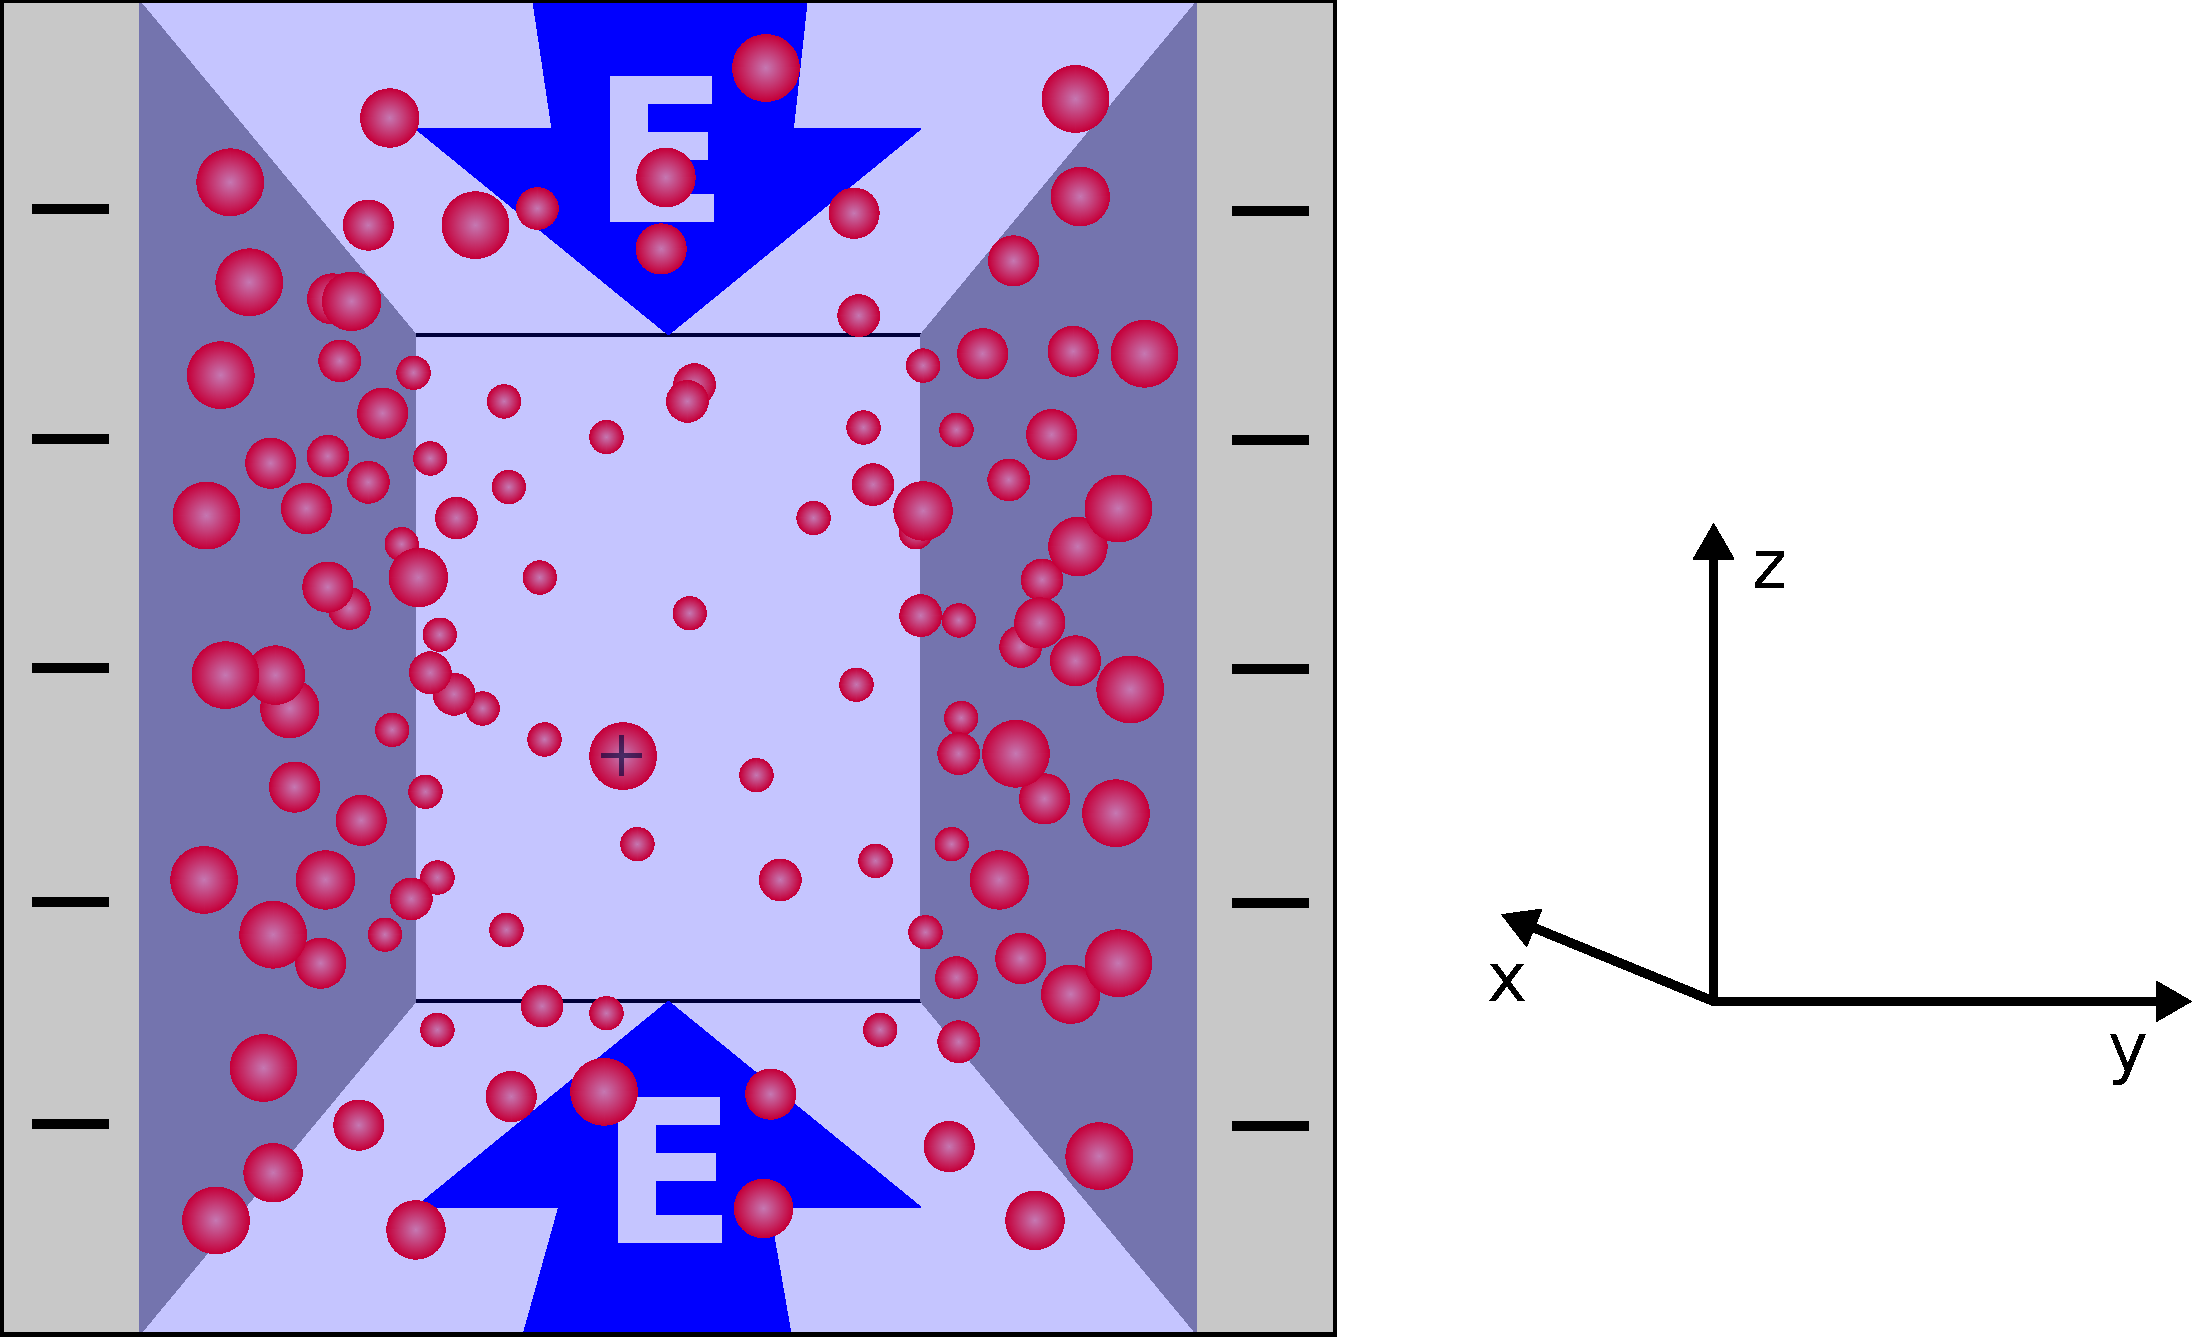
\includegraphics[width=0.5\columnwidth]{figures/schlitzpore_3d.pdf}
\end{center}
\pagebreak
\definecolor{mygray}{gray}{.75}
\begin{center}
  \colorbox{mygray}{ 
\begin{minipage}[h]{13cm}
  \textbf{\large Before you start:}\\
  With this tutorial you can get started using the Lattice-Boltzmann method
  for scientific applications. We give a brief introduction about the theory
  and how to use it in \ES{}. 
  We have selected three interesting problems for which LB can be applied
  and which are well understood.  You can start with any of them.
   

  The tutorial is relatively long and working through it carefully
  is work for at least a full day. You can however get a glimpse 
  of different aspects by starting to work on the tasks.


  Note: LB can not be used as a black box. It is unavoidable 
  to spend time learning the theory and gaining practical experience. 
\end{minipage}
}
\end{center}

 \tableofcontents
 \pagebreak
  
\section{Introduction}

%\floatingBox{5}{4cm}{Mein Text der in der Box abgebildet werden soll. Mal schauen wie das klappt.} 


In this tutorial, you will learn basics about the 
Lattice Boltzmann Method (LBM) with special focus on the application
on soft matter simulations or more precisely on how to apply it 
in combination with molecular dynamics to take into account 
hydrodynamic solvent effects without the need to introduce
thousands of solvent particles. 

The LBM -- its theory as well as its applications -- is 
still a very active field of research. After almost 20 years
of development there are many cases in which the LBM has proven
to be fruitful, in other cases the LBM is considered promising,
and in some cases it has not been of any help. We
encourage you to contribute to the scientific discussion 
of the LBM because there is still a lot 
that is unknown or only vaguely known about this fascinating
method. 

\subsection*{Tutorial Outline}
This tutorial should enable you to start a scientific project applying
the LB method with \ES{}. In the first part we summarize a few basic ideas behind LB 
and describe the interface. In the second part we suggest three
different classic examples where hydrodynamics are important. These are
\begin{itemize}
  \item \textbf{Hydrodynamic resistance of settling particles.} We measure the drag
   force of single particles and arrays of particles when sedimenting
   in solution.
  \item \textbf{Polymer diffusion.} We show that the diffusion of polymers is accelerated 
    by hydrodynamic interactions.
  \item \textbf{Poiseuille flow.} We reproduce the flow profile between two walls.
\end{itemize}

\subsection*{Notes on the \ES{} version you will need}
With Version 3.1 \ES{} has learned GPU support for LB. We recommend however
version 3.3, to have all features available. We absolutely recommend using 
the GPU code, as it is much (100x) faster than the CPU code.

For the tutorial you will have to compile in the following  features:
\texttt{PARTIAL\_PERIODIC}, \texttt{EXTERNAL\_FORCES}, \texttt{CONSTRAINTS}, \texttt{ELECTROSTATICS}, 
\texttt{LB\_GPU}, \texttt{LB\_BOUNDARIES\_GPU},  \texttt{LENNARD\_JONES}.

All necessary files for this tutorial are located in the directory
\texttt{espresso/doc/tutorials/python/04-lattice\_boltzmann/scripts}.
\pagebreak


